%%%%%%%%%%%%%%%%%%%%%%%%%%%%%%%%%%%%%%%%%%%%%%%%%%%%%%
%% Slides : Introduction to probabilistic reasoning %%
%%%%%%%%%%%%%%%%%%%%%%%%%%%%%%%%%%%%%%%%%%%%%%%%%%%%%%

%% PREAMBLE
%% Define document class and basic options
\documentclass{beamer}
%\setlength{\parindent}{0pt}

%% Load packages
\usepackage{palatino}
\usepackage{amsfonts}
\usepackage{amsmath}
%\usepackage{url}
\usepackage{hyperref}
%\usepackage{listings}
\usepackage{verbatim}
\usepackage[utf8]{inputenc} %% For french
\usepackage{tikz} %% For drawing (eg, Venn diagrams)
\usefonttheme{serif}

\hypersetup{
	colorlinks=true,
	linkcolor=blue,
	citecolor=red,
	filecolor=blue,
	urlcolor=blue
}

\usetheme{Madrid}

%% Basic info
\title{Introduction à la pensée et aux méthodes en probabilité}
%\subtitle{}
\author{Roy Nitulescu\inst{1}}

\institute
{
    \inst{1}%
    CITADEL\\
    CR-CHUM
}

\date[UdeM, Sept. XX, 2023]{Université de Montréal, Sept. XX, 2023}

\AtBeginSection[]
{
    \begin{frame}
        \frametitle{Table des matières}
        \tableofcontents[currentsection]
    \end{frame}
}

\AtBeginSubsection[]
{
    \begin{frame}
        \frametitle{Table des matières}
        \tableofcontents[currentsubsection]
    \end{frame}
}


%% BEGIN DOCUMENT
\begin{document}

%%%%
%% Slides
%%%%

\frame{\titlepage}

\begin{frame}
    \frametitle{Épigraphe}
    ``La probabilité est le concept le plus important de la science moderne,
    d'autant plus que personne n'a la moindre idée de ce qu'elle signifie.'' -- Bertrand Russell, 1929
\end{frame}


\begin{frame}
    \frametitle{Préambule}
    
    Le code source pour cette présentation ce trouve ici:

    \vfill

    \url{https://github.com/rnitulescu/prob2023}
\end{frame}


\begin{frame}
    \frametitle{Table des matières}
    \tableofcontents
\end{frame}


%%%%
%% Le raisonnement
%%%%

\section{Le raisonnement}

\begin{frame}
    \frametitle{Le raisonnement}
    \textbf{Définition:}\

    \bigskip

    Le \emph{raisonnement} c’est la combinaison d’informations dans le
    but d’aboutir à une conclusion qui est liée à ces informations.\\

    \vfill \pause

    \textbf{Types de raisonnement:}\\

     par deduction \pause, par abduction \pause, par induction
\end{frame}


\begin{frame}
    \frametitle{Le raisonnement par déduction}
    \begin{itemize}
      \item Une approche \emph{formelle} de raisonnement \pause
      \item Commence avec des \emph{prémisses} \pause
      \item Le processus avance par l’application de règles formelle \emph{d’inférence} \pause
      \item Aboutit à une conclusion qui suit de façon \emph{nécessaire} des prémisses \pause
      \item Ne permet pas d’aboutir à des conclusions qui ne sont pas déjà
            implicites dans les prémisses (donc \emph{non-ampliatif})
    \end{itemize}
\end{frame}


\begin{frame}
    \frametitle{Exemples de déduction}
    \textbf{Ex 1:}\\ \pause
    \emph{Prémisse:} Tout les hommes sont mortels\\ \pause
    \emph{Prémisse:} Socrate est un homme\\ \pause
    \emph{Conclusion:} Socrate (étant un homme) est lui aussi mortel\

    \bigskip \pause

    \textbf{Ex 2:}\\
    Toute preuve mathématique
\end{frame}


\begin{frame}
    \frametitle{Le raisonnement par abduction}
    \begin{itemize}
      \item Approche \emph{informelle} de raisonnement \pause
      \item Commence avec un ensemble \emph{limité} d’observations \pause
      \item Le but est de trouver \emph{l’explication} la plus \emph{probable} des faits observés \pause
      \item La conclusion \emph{ne suit pas} de façon nécessaire des faits (donc incertain) \pause
      \item Permet d’aboutir à des explications qui ne sont pas
            implicites dans les faits (donc \emph{ampliatif})
    \end{itemize}
\end{frame}


\begin{frame}
    \frametitle{Exemples d'abduction}
    \textbf{Ex 1:}\\ \pause
    \emph{Fait:} Le sol est mouillé tout autour de ma maison\\ \pause
    \emph{Fait:} Le sol n'est pas mouillé autour des maisons de mes voisins\\ \pause
    \emph{Explications probables:}\\ \pause
          (1) Il y a eu de la pluie seulement au dessus de ma maison,\\ \pause
          (2) J'ai oublié d'éteindre mes arroseurs de jardin\\ \pause

    \smallskip

    \emph{Explication la plus probable:} J'ai oublié d'éteindre mes arroseurs de jardin\

    \bigskip \pause

    \textbf{Ex 2:}\\
    Travail de détectives policiers, diagnostics médicaux
\end{frame}


\begin{frame}
    \frametitle{Le raisonnement par induction}
    \begin{itemize}
      \item Approche \emph{informelle} de raisonnement \pause
      \item Commence avec un ensemble d’observations \pause
      \item Le but est de \emph{généraliser} à partir des faits observés \pause
      \item Le plus qu’on a d’observations fait sous des conditions homogènes,
            le plus probable nos conclusions \pause
      \item La conclusion \emph{ne suit pas} de façon nécessaire des faits (donc incertain) \pause
      \item Permet d’aboutir à des explications qui ne sont pas
            implicites dans les faits (donc \emph{ampliatif})
    \end{itemize}
\end{frame}


\begin{frame}
    \frametitle{Exemples d'induction}
    \textbf{Ex 1:}\\ \pause
    \emph{Observations:} Le soleil c’est levé et c’est couché à chaque jour de ma vie \pause
    \emph{Généralisation:} Le soleil ce lève et ce couche à chaque jour\

    \bigskip \pause

    \textbf{Ex 2:}\\
    Moyen d’apprentissage des enfants, études cliniques
\end{frame}


\begin{frame}
    \frametitle{Propriétées des différents types de raisonnement}
    \begin{center}
      %\begin{tabular}{ | l | c c c | }
      \begin{tabular}{ | p{0.14\linewidth} | p{0.24\linewidth} | p{0.24\linewidth} | p{0.24\linewidth} | }
        \hline \hline
         & Déduction & Abduction & Induction \\
        \hline \hline
        Procédure & Raisonnement à partir de prémisses pour aboutir à une conclusion via des règles \emph{formelles} d'inférence
                  & Raisonnement à partir d'observations incomplètes pour aboutir à \emph{l'explication}
                    la plus probable de ces observations
                  & Raisonnement à partir de maintes observations pour aboutir à une \emph{généralisation}
                    (que les prochaines observations seront semblables)
                  \\
        \hline
        Nécessaire & Oui (certain) & Non (incertain) & Non (incertain) \\
        \hline
        Ampliatif & Non & Oui & Oui \\
        \hline \hline
      \end{tabular}
    \end{center}
\end{frame}


%%%%
%% Intuition à propos de la probabilité
%%%%

\section{Intuition à propos de la probabilité}

%% Monty Hall problem
%\subsection{Le problème \emph{Monty Hall}}

\begin{frame}
    \frametitle{Le problème \emph{Monty Hall}}
    \emph{
    ``Vous participez à un jeu télévisé.
    L’animateur vous demande de choisir une porte parmi les trois possibles.
    Le lot gagnant se trouve derrière seulement une des trois portes.
    Une fois votre choix fait, l’animateur ouvre une des trois portes.
    Mais pour garder le suspense, l’animateur n’ouvre ni la porte que
    vous avec choisi, ni la porte gagnante.
    Finalement, l’animateur vous demande si vous voudriez changer de choix
    pour l’autre porte qui n’est pas encore ouverte.''}\\

    \bigskip \pause

    \textbf{La question:} Quel est la meilleure stratégie?
    Est-ce que vous ‘changez’ ou est-ce que vous ‘restez’?\\

    \bigskip \pause

    Ce problème est assez célèbre. Il a été sujet de débats et de controverses.
    Vous pouvez en apprendre plus sur la page Wikipédia:
    \url{https://en.wikipedia.org/wiki/Monty_Hall_problem}
\end{frame}


\begin{frame}
    \frametitle{Solution au problème \emph{Monty Hall}}
    De quelle information est-ce qu’on aurait besoin pour faire un choix éclairé?\\

    \bigskip \pause

    Si on savait que le lot gagnant était derrière notre premier choix de porte,
    on ne changerait pas de choix.\\ %Et vice-versa, si on savait que le lot gagnant
    %n’était pas derrière notre premier choix de porte, alors on changerait de choix.\\

    \bigskip \pause

    Mais, puisqu’il y a \emph{une chance sur trois} qu’on a choisi la bonne porte au début,
    si on choisi de ‘rester’, on gagnera seulement \emph{une fois sur trois}.\\

    \bigskip \pause

    Voici un diagramme des possibilités.
\end{frame}


\begin{frame}
    \begin{figure}
      \centering
      \scalebox{0.60}{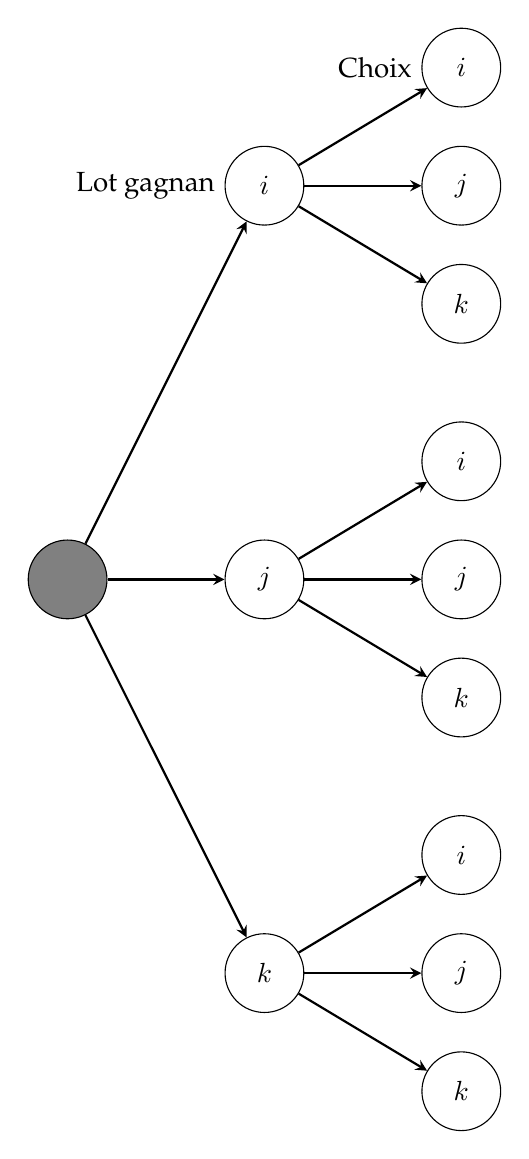
\begin{tikzpicture}
    \tikzstyle{arrow} = [thick,->,>=stealth]
    % Left-most circle
    \node [draw, circle, minimum size=1cm, fill=gray] (Left) at (-5,0) {};

    % One step to the right, top circle
    \node [draw, circle, minimum size=1cm, text centered, label={-180:Lot gagnan}] (MidTop) at (-2.5,5) {$i$};
    \draw [arrow] (Left) -- (MidTop);

      % Two steps to the right, MidTop is parent, top circle
      \node [draw, circle, minimum size=1cm, text centered, label={-180:Choix}] (MidTopTop) at (0,6.5) {$i$};
      \draw [arrow] (MidTop) -- (MidTopTop);

      % Two steps to the right, MidTop is parent, mid circle
      \node [draw, circle, minimum size=1cm] (MidTopMid) at (0,5) {$j$};
      \draw [arrow] (MidTop) -- (MidTopMid);

      % Two steps to the right, MidTop is parent, bottom circle
      \node [draw, circle, minimum size=1cm] (MidTopBottom) at (0,3.5) {$k$};
      \draw [arrow] (MidTop) -- (MidTopBottom);

    % One step to the right, middle circle
    \node [draw, circle, minimum size=1cm] (MidMid) at (-2.5,0) {$j$};
    \draw [arrow] (Left) -- (MidMid);

      % Two steps to the right, MidMid is parent, top circle
      \node [draw, circle, minimum size=1cm] (MidMidTop) at (0,1.5) {$i$};
      \draw [arrow] (MidMid) -- (MidMidTop);

      % Two steps to the right, MidMid is parent, mid circle
      \node [draw, circle, minimum size=1cm] (MidMidMid) at (0,0) {$j$};
      \draw [arrow] (MidMid) -- (MidMidMid);

      % Two steps to the right, MidMid is parent, bottom circle
      \node [draw, circle, minimum size=1cm] (MidMidBottom) at (0,-1.5) {$k$};
      \draw [arrow] (MidMid) -- (MidMidBottom);

    % One step to the right, bottom circle
    \node [draw, circle, minimum size=1cm] (MidBottom) at (-2.5,-5) {$k$};
    \draw [arrow] (Left) -- (MidBottom);

      % Two steps to the right, MidBottom is parent, top circle
      \node [draw, circle, minimum size=1cm] (MidBottomTop) at (0,-3.5) {$i$};
      \draw [arrow] (MidBottom) -- (MidBottomTop);

      % Two steps to the right, MidBottom is parent, mid circle
      \node [draw, circle, minimum size=1cm] (MidBottomMid) at (0,-5) {$j$};
      \draw [arrow] (MidBottom) -- (MidBottomMid);

      % Two steps to the right, MidBottom is parent, bottom circle
      \node [draw, circle, minimum size=1cm] (MidBottomBottom) at (0,-6.5) {$k$};
      \draw [arrow] (MidBottom) -- (MidBottomBottom);
\end{tikzpicture}

}
    \end{figure}
\end{frame}


\begin{frame}
    \begin{figure}
      \centering
      \scalebox{0.60}{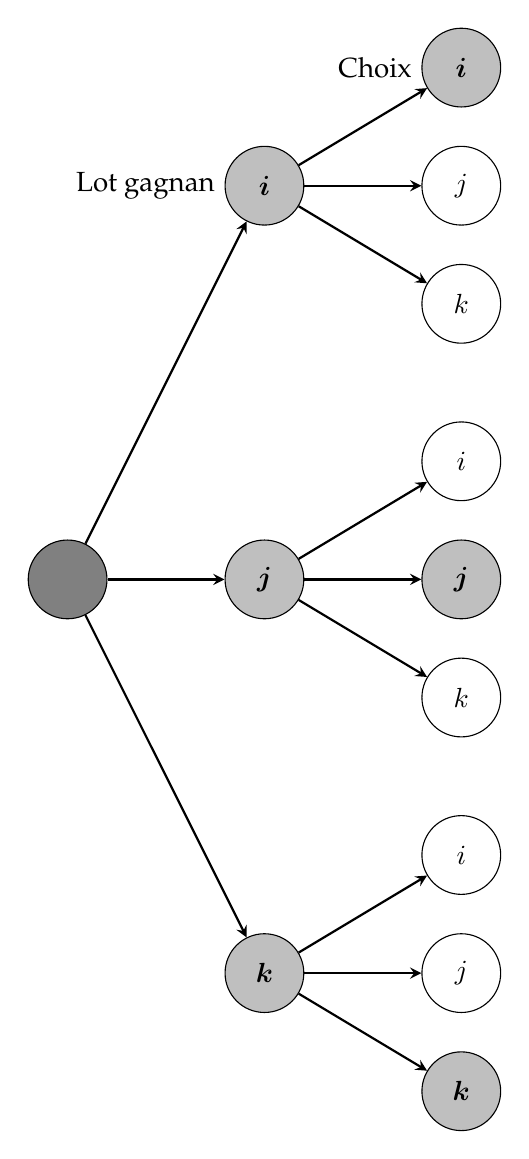
\begin{tikzpicture}
    \tikzstyle{arrow} = [thick,->,>=stealth]
    % Left-most circle
    \node [draw, circle, minimum size=1cm, fill=gray] (Left) at (-5,0) {};

    % One step to the right, top circle
    \node [draw, circle, minimum size=1cm, fill=lightgray, text centered,
           label={-180:Lot gagnan}] (MidTop) at (-2.5,5) {{$\boldsymbol{i}$}};
    \draw [arrow] (Left) -- (MidTop);

      % Two steps to the right, MidTop is parent, top circle
      \node [draw, circle, minimum size=1cm, fill=lightgray, text centered,
             label={-180:Choix}] (MidTopTop) at (0,6.5) {$\boldsymbol{i}$};
      \draw [arrow] (MidTop) -- (MidTopTop);

      % Two steps to the right, MidTop is parent, mid circle
      \node [draw, circle, minimum size=1cm] (MidTopMid) at (0,5) {$j$};
      \draw [arrow] (MidTop) -- (MidTopMid);

      % Two steps to the right, MidTop is parent, bottom circle
      \node [draw, circle, minimum size=1cm] (MidTopBottom) at (0,3.5) {$k$};
      \draw [arrow] (MidTop) -- (MidTopBottom);

    % One step to the right, middle circle
    \node [draw, circle, minimum size=1cm, fill=lightgray] (MidMid) at (-2.5,0) {$\boldsymbol{j}$};
    \draw [arrow] (Left) -- (MidMid);

      % Two steps to the right, MidMid is parent, top circle
      \node [draw, circle, minimum size=1cm] (MidMidTop) at (0,1.5) {$i$};
      \draw [arrow] (MidMid) -- (MidMidTop);

      % Two steps to the right, MidMid is parent, mid circle
      \node [draw, circle, minimum size=1cm, fill=lightgray] (MidMidMid) at (0,0) {$\boldsymbol{j}$};
      \draw [arrow] (MidMid) -- (MidMidMid);

      % Two steps to the right, MidMid is parent, bottom circle
      \node [draw, circle, minimum size=1cm] (MidMidBottom) at (0,-1.5) {$k$};
      \draw [arrow] (MidMid) -- (MidMidBottom);

    % One step to the right, bottom circle
    \node [draw, circle, minimum size=1cm, fill=lightgray] (MidBottom) at (-2.5,-5) {$\boldsymbol{k}$};
    \draw [arrow] (Left) -- (MidBottom);

      % Two steps to the right, MidBottom is parent, top circle
      \node [draw, circle, minimum size=1cm] (MidBottomTop) at (0,-3.5) {$i$};
      \draw [arrow] (MidBottom) -- (MidBottomTop);

      % Two steps to the right, MidBottom is parent, mid circle
      \node [draw, circle, minimum size=1cm] (MidBottomMid) at (0,-5) {$j$};
      \draw [arrow] (MidBottom) -- (MidBottomMid);

      % Two steps to the right, MidBottom is parent, bottom circle
      \node [draw, circle, minimum size=1cm, fill=lightgray] (MidBottomBottom) at (0,-6.5) {$\boldsymbol{k}$};
      \draw [arrow] (MidBottom) -- (MidBottomBottom);
\end{tikzpicture}

}
    \end{figure}
\end{frame}


\begin{frame}
    \frametitle{Solution au problème \emph{Monty Hall}}
    Dans l’état 1 (‘on a choisi la bonne porte’),
    on gagne avec certitude si on ‘reste’ (3 cas sur 9).\\

    \vfill \pause

    Dans l’état 2 (‘on a choisi une des mauvaises portes’),
    on gagne avec certitude si on ‘change’ (6 cas sur 9).\\

    \vfill \pause

    Notre hypothèse (très raisonnable) est que \emph{a priori}:
    \begin{enumerate}
      \item toutes les trois portes ont une chance égale de cacher le lot gagnant
      \item on n’a aucune préférence particulière pour faire notre choix de porte
    \end{enumerate}

    \vfill \pause

    Puisque les neuf possibilités sont équiprobables, par nos hypothèses, on à notre réponse:\\

    \vfill \pause

    On est mieux de \emph{changer}, peut-importe notre choix initial,
    puisque cela nous donne \textbf{6} chances sur \textbf{9} de gagner
    versus les \textbf{3} chances sur \textbf{9} si on \emph{reste}.
\end{frame}


\begin{frame}
    \frametitle{Solution au problème \emph{Monty Hall}}
    Caractéristiques du problème qu’on vient de résoudre: \pause
    \begin{itemize}
      \item On connais les chances de gagner (les règles du jeu) \pause
      \item On est incertain à propos de notre décision de quelle porte choisir au début  \pause
      \item Ensuite on est incertain à propos de la meilleure stratégie (‘rester’ ou ‘changer’)  \pause
      \item Mais, on à été capable de \emph{déduire} quelle était la meilleure stratégie,
            \emph{en connaissant les règles du jeu}
    \end{itemize}

    \vfill \pause

    Les premières applications qui on donnés naissance au concept et
    à la théorie de la probabilité en Europe étaient des questions à propos
    des jeux de hasard (ex: correspondance entre Fermat et Pascal au 17\textsuperscript{e} siècle)
\end{frame}


%%%%
%% Le concept de la probabilité
%%%%

\section{Le concept de probabilité}

\begin{frame}
    \frametitle{La dualité du concept de probabilité}

    De par son origine, le concept a une \textbf{dualité}\footnote{
    Hacking, Ian (1975). \emph{The emergence of probability:
    A philosophical study of early ideas about probability,
    induction and statistical inference}. Cambridge University Press.
    }

    \pause

    \vfill

    \begin{enumerate}
      \item \textbf{Aléatoire}
        \begin{itemize}
          \item Fréquence (la limite d'une fréquence relative dans une séquence infinie)
          \item Propension (une propriété intrinsèque d'objets ou de situations)
        \end{itemize}

      \pause

      \item \textbf{Épistémique}
        \begin{itemize}
          \item Logique (le degré de soutien ou de confirmation qu'un élément d'évidence confère à une hypothèse donnée)
          \item Subjectif (crédibilité ou degré de croyance subjectif)
        \end{itemize}
    \end{enumerate}
\end{frame}






%% Tentative sections...
\section{Le calcul de probabilité}

\section{L'inférence probabiliste}

\subsection{Incertitude due à l'aléa des observations}%% binomial & negative binomial examples?
%% also some typical frequentist tests, like the Student's t-test

\subsection{Incertitude due à un manque de connaissance}%% recall Monty Hall problem (maybe show formal prob. theory solution.)
%% monty hall case, the categorial parameter is unknown. But we can have unknown continuous parameters, etc.

\subsection{Incertitude due aux deux}

%% what we take as known, what we take as unknown...

%% Idea: maybe illustrate each application area with simple, accessible examples, and then show that
%%       this is what is done when we use more advanced standard procedures that often require specialized software?

%% Do we cover CLT, estimation theory (bias, MSE, MM, ML)???

%% I want to maximize the conceptual content, and not focus as much on the technical depth
%% But I also want to show some cool stuff like CLT and Laplace approximaiton (a way to also derive the Normal pdf...)


%% END DOCUMENT
\end{document}

